\scanpage{56}
% archive sheet number: 55

% Top left, loose mark
\margin{$X$}

% L1–4, upper left
\figure{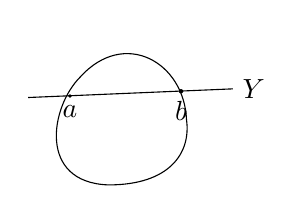
\begin{tikzpicture}[x=1cm,y=1cm]\draw (0,-.55) .. controls (-.90,-.52) and (-.74,.44) .. (-.36,.82) .. controls (.20,1.44) and (.96,1.01) .. (.99,.28) .. controls (1.05,-.15) and (.77,-.55) .. (0,-.55);\draw (-1.02,.56)--(1.58,.67) node[right] {$Y$};\fill (-.49,.58) circle (.024) node[below] {$a$};\fill (.92,.64) circle (.028) node[below] {$b$};\end{tikzpicture}}

% L1–8, following Ex 2
Considérons $X_1={}$ cercle cf figure, et le faisceau $F_1$ \inserted{sur $X_1$} des applications dans $\mathbb{Q}$, soit $F$ son image sur $X$. La question de prolonger une section sur $Y$ à $X$ est équivalente à celle de prolonger une section sur $Y\cap X_1$ à $X_1$, \uline{or on a} vu que c'est en général impossible.

% L9–12, third example
\uline{Ex 3} Un faisceau induit par un injectif n'est généralement pas flasque \inserted{(ni mou)} ; les \inserted{Exemples 1 et 2 prouvent qu'un faisceau \deleted{flasque} \inserted{injectif donc flasque} n'est pas néc. mou, donc il \unsure{n'y a qu'à prendre|n'y a qu'à faire} $X=Y$]} \deleted{de façon précise, dans le cas de l'ex 2, le faisceau $F|Y$}

% L13–15, cancelled paragraph
\deleted{Soient $X,Y$ comme dans l'exemple 2, $F$ étant cette fois ci le faisceau des applications de $X$ dans $\mathbb{Q}$,}

% L16–20, lower right
On ne s'en tire pas \unsure{sur|pour} $Y$ une courbe \uline{irréductible} [\unsure{ici|car|i.e.}, \unsure{ds ce cas} le faisceau induit est tjrs flasque, facile].

% L16–19, lower left
\figure{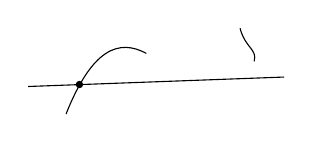
\begin{tikzpicture}[x=1cm,y=1cm]\draw (0,0)--(3.25,.12);\draw (.48,-.35) .. controls (.81,.48) and (1.15,.61) .. (1.50,.42);\fill (.65,.025) circle (.047);\draw[thin] (2.69,.74) .. controls (2.76,.48) and (2.91,.48) .. (2.87,.32);\end{tikzpicture}}

% L21–23, foot
Mais prenons pour $Y$ la réunion de 2 courbes \inserted{$Y_1$ et $Y_2$ \deleted{\unsure{ds}}} se coupant en $\unsure{0|a}$, dans $X$ \inserted{\uline{irréd}}
